\chapter{Motivation}
\label{chap:motivation}
The initial version of the learning environment (LDBN 1.0) was used in
conjunction with the course \emph{Principles of Database Systems} at the 
Department of Computing Science at the Ume� University, and some important 
observations were made. In this chapter we present the problems with the 
LDBN 1.0, which were observed during this testing period. 
Some of the problems led to the realization that the learning environment needs to be further developed 
%ne mi haresva
and extended in order to allow a more extensive and productive use 
of the system, and in order for the students to be assisted even better 
in the process of understanding the concepts of FDs and 
relational-database normalization by providing new tools to them such as the 
FD visualization tool, which is described in detail in Section~\ref{sec:visualization}.  

\section{Problem Statement}
\label{sec:problem_statement}
At the moment, students, who are trying to solve an assignment with LDBN, often have
to deal with a large number of attributes and FDs based on those attributes. 
However, LDBN 1.0 offers only textual representation of FDs, an example of such
representation is shown in Figure~\ref{fig:exampleFds01} . 

\begin{figure}[h]
	\begin{center}
		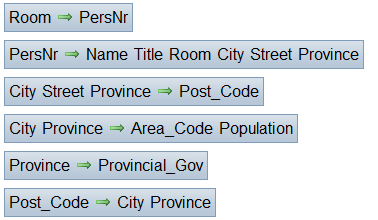
\includegraphics[width=0.7\textwidth]{./img/example_fds_01.png}
		\caption{Example of a Typical Textual Representation of FDs in LDBN 1.0}
		\label{fig:exampleFds01}
	\end{center}
\end{figure}


As can be seen, some attributes 
may occur more than once in a single FD and there may be many different FDs in a single 
assignment. Although this is a standard representation of FDs, 
it may lead to a confusion among students and negatively affect the overall
usability of the system. Thus we extended LDBN 1.0 by providing a visualization for
FDs. In order the visualization to be intuitive for 
both students and lecturers we have decided to use templates found in popular 
popular database textbooks such as~\cite{bdb2} and~\cite{bdb1}. 
An example of a such visualization can be observed in Figure~\ref{fig:viz-fds-ex01}, which
was generated with LDBN 1.1. 

\begin{figure}[h]
	\begin{center}
		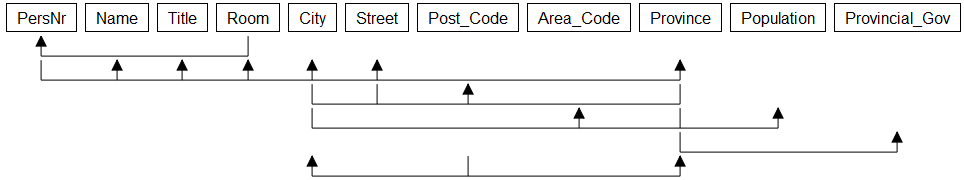
\includegraphics[width=0.95\textwidth]{./img/example_fds_02.png}
		\caption{Example of a Graphical Representation of FDs in LDBN 1.1}
		\label{fig:viz-fds-ex01}
	\end{center}
\end{figure}

Another example of the new visualization functionality can be observed in Figure~\ref{fig:viz-fds-ex02}. 
Figure~\ref{fig:viz-fds-ex02a} shows a set of FDs represented as text in LDBN 1.0, 
and Figure~\ref{fig:viz-fds-ex02b} shows the same set of FDs using the visualization functionality of LDBN 1.1.
The Example is an adaptation of~\cite[Aufgabe~6.7]{bdb2ub}. 
In this case the visualization clearly stands out,
as it delivers a much clearer overview of the FD set. For instance, with the help of the 
visualization one can clearly see that some FDs are redundant, such as $A \rightarrow B$ or $E \rightarrow B C$.
In fact for relatively small sets of FDs, which are typical for LDBN, by using the visualization functionality 
one can easily apply Algorithm~4.12 in~\cite{mt1}, which is used for computing a minimal cover of an FD set -~$F_c$.
In this case a minimal cover may be defined as  
$F_c = A \rightarrow B; E \rightarrow A; F \rightarrow C D; C \rightarrow B E F$. 
Thus all other FDs are redundant, as they may be inferred from $F_c$. 
Readers unfamiliar with the term \emph{Minimal Cover of an FD Set} may refer to~\cite[Section~2.1.6]{mt1}. 

\begin{figure}[h]
  \centering
  \subfigure[Textual Representation]{
    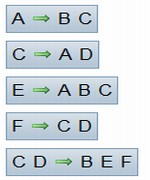
\includegraphics[scale=0.7]{./img/ldbn-viz-ex-fc00.jpg}
    \label{fig:viz-fds-ex02a}
  }
  \subfigure[Graphical Representation]{
    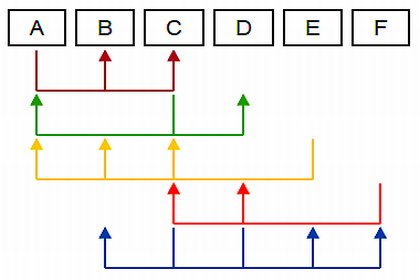
\includegraphics[scale=0.45]{./img/ldbn-viz-ex-fc01.jpg}
    \label{fig:viz-fds-ex02b}
  }
\caption{Example of Different Types of Representation of FDs in LDBN}
\label{fig:viz-fds-ex02}
\end{figure}   

Another major problem with the initial system is the fact that all 
registered users have the same rights. Thus all users can create assignments, which
can be seen by all other registered or unregistered users. In addition, assignments
can be viewed in the \emph{Solve Assignment Tab} only if they have been previously
stored in the system by a registered user. In the original version of the environment (LDBN 1.0),
it was believed that both of these facts would increase the number and the diversity of
assignments stored in the systems, and thus the system would appeal to more students 
and increase usability. 
This collaborative approach has been inspired by the Wikipedia project, where everyone
can be a content contributor and a reader at the same time. 
However, during the testing period the system has been flooded with unsuitable assignments
mainly because of two reasons. First, 
identical assignments occurred more than once under different names. They were usually submitted 
by students in the same class trying to
solve a homework assignment, or just trying the system with examples from textbooks.
Second, users were unable to load an assignment in the \emph{Solve Assignment Tab}
without first storing it in the database of the system, this led to the fact that
users who just wanted to test the system with a simple assignment were in fact
flooding LDBN 1.0 with even more unsuitable assignments, which consist of just a 
few attributes and even less FDs, and were of no interest to other users. Both of these
facts led to a major decrease in the usability of the system, 
since students were no longer able to distinguish 
between interesting and well-thought-out assignments submitted by lecturers 
and other assignments.
 
To solve the above problem a more sophisticated user system was introduced. In the 
current version of the learning environment (LDBN 1.1) users are basically dividend into two groups - 
regular users (students) and instructional users (lecturers).
First, instructional users
have more rights than regular users. Second, only assignments submitted by instructional users
are visible by default.  
In addition, lecturers have many more rights in the system than students.
This is discussed in detail in Section~\ref{sec:improving}. 
 

\section{Purpose}
\label{sec:purpose}
The purpose of this thesis can be divided into two parts:

\begin{enumerate}

  \item Implementing different types of visualization for FDs based 
  on templates found in popular textbooks such as~\cite{bdb2} and~\cite{bdb1}. 
  Furthermore, the visualization should support different colors schemata and 
  zoom levels for a better presentation. Furthermore, the visualization
  should be available in all fields of the UI which hold a set of FDs. 
  In addition to this, it should not interfere with existing representation of the FDs.

  \item Improving the existing system in several ways including:
  
  \begin{enumerate}
    \item Dividing the user into at least two groups: 
    (1) instructional users and (2) regular registered users. This is done without
    affecting the existing users, thus all already registered users will keep
    their rights in the system. 
    \item Decrease the number arbitrary assignments by providing new methods for saving and 
    loading assignments in the system. 
    \item Users should be able to delete and edit their previously submitted comments.    
  \end{enumerate}
  
\end{enumerate}

%TODO some more motivation so you can get four pages for this chapter
 